\documentclass[titlepage]{article}

\usepackage{graphicx}
\usepackage{tabularx}
\graphicspath{{./figures}}

\title{%
    Engineering Physics 353 Final Report \\
    \large Team 14 - ``Team 4"}
\author{Nathan Van Rumpt, Eric Souder}
\date{April 2023}

\begin{document}
\maketitle

\begin{abstract}
    This is the abstract.
\end{abstract}

\section{Background}

\section{Overall Architecture}

\section{Navigation}
    Robot navigation was accomplished with an almost entirely classical control system, using minimal neural network-based approaches and instead using manually-tuned computer vision and classical control techniques. 

    The navigation controller was composed of two ROS nodes: The `State Machine' node was composed of a finite state machine and the `Navigate' node contained a set of navigation algorithms for different scenarios, selecting an appropriate algorithm based on the state reported by the state machine. States were communicated internally between the two nodes via a ROS topic.
    
    \subsection{State Machine}
        The finite state machine responsible for controlling the robot's navigation state was composed primarily of a number of state classes, representing a unique navigational state and a state machine class responsible for orchestrating the transitions between them. Each state class, such as the `Pave Navigate' or `Junction Wait' states, is a subclass of an abstract parent class which defines an `evaluate transition' interface responsible for determining the next state to enter and either returns itself to remain in the current state or generates a new state object to transition into. The state machine class calls this method each frame to determine which state the robot should be in, and then broadcasts that state to the navigation node via a ROS topic. The overall state machine diagram is shown in Figure~\ref{fig:statemachine}.

        \begin{figure}
            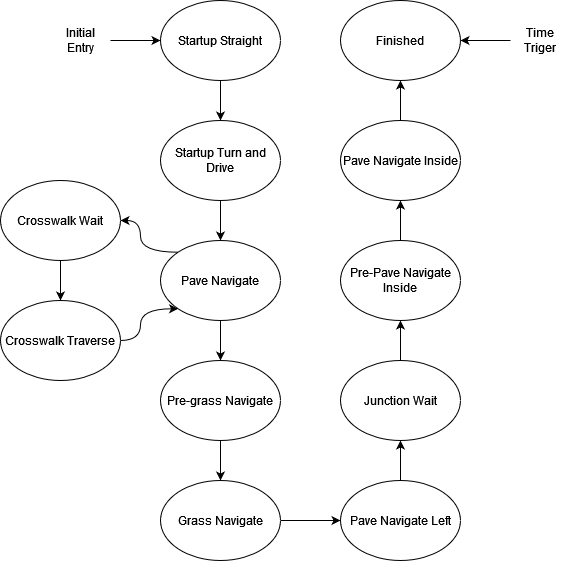
\includegraphics[width=\linewidth]{statemachine.png}
            \caption{Diagram of the robot state machine.}
            \label{fig:statemachine}
        \end{figure}

        Three main types of navigational states existed: active navigation states, stopped states, and preprogrammed states. In preprogrammed states, where the robot executes a constant movement, the state machine transitions based off of a simple timer to move to the next state once the movement had been in progress for the preprogrammed length of time. In active navigation states, where the navigation algorithm is interpreting each frame on the fly to determine a which movement to command, or in stopped states, where the robot is waiting for an event to occur before proceeding, the state machine interpets each frame and makes a transition decision based on it.

        \subsubsection{Pavement and Grass Detection}
            In order to transition from the pavement navigation states to the grass navigation state and vice versa, the state machine must be able to determine if the robot is driving on grass or on pavement. This detection is accomplished with a small neural network, implemeted within a `SurfaceDetector' class. Training data was 400 images captured from the robot camera, evenly split between grass and pavement surfaces. Data was aqquired by by manually driving the vehicle around with a simple ros node activated to save each camera frame. Because of the goal of simplicity for the neural network, all images were preprocessed by signifigant compression, images were resized to 0.025 times their original width and 0.05 times their original height, this resulted in a 36 by 32 image, which was further cropped to remove the top 18 rows of pixels, focusing only on the ground and removing the area above the horizon.

            The simple model was composed of only three layers: An input flatten layer, a hidden dense layer, and a output dense layer composed of a single neuron, with a total of 2,666,689 trainable parameters, as shown in Figure~\ref{fig:surfacedetectmodel}.
            \begin{figure}
                \begin{tabularx}{0.9\linewidth}{ 
                     >{\raggedright\arraybackslash}X 
                     >{\raggedright\arraybackslash}X 
                     >{\raggedleft\arraybackslash}X  }

                     Layer (type) & Output Shape & Num. Params. \\ 
                    \hline \\
                    Flatten & (None, 1632) & 0 \\  
                    Dense & (None, 1632) & 2665056 \\
                    Dense & (None, 1) & 1633 \\
                \end{tabularx}
                \caption{Summary of surface detection neural network}
                \label{fig:surfacedetectmodel}
            \end{figure}
            The model was trained with a learning rate of $1 \times 10^{-4}$ and a validation split of 0.2 over 10 epochs. Loss and accuracy curves by epoch are shown in Figure~\ref{fig:grasspavegraphs}.

            \begin{figure}
                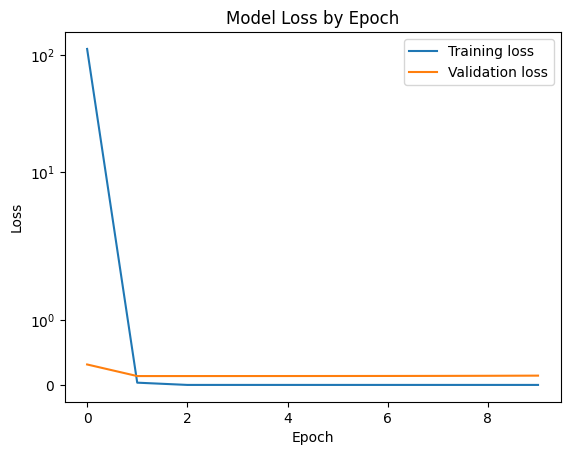
\includegraphics[width=\linewidth]{grasspaveloss.png}
                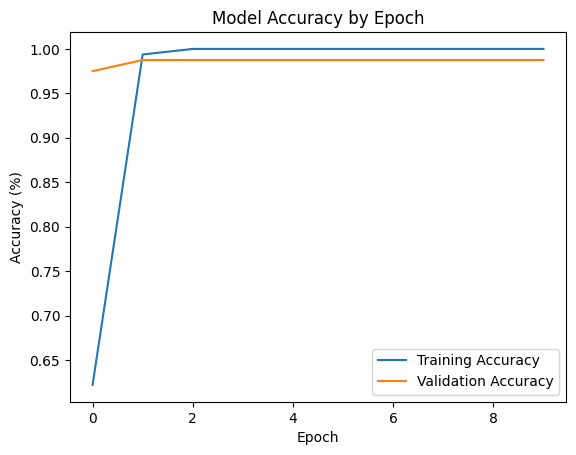
\includegraphics[width=\linewidth]{grasspaveacc.png}
                \caption{Loss and accuracy of grass and pavement detection network by training epoch.}
                \label{fig:grasspavegraphs}
            \end{figure}

            Because of the small size and binary output of the network, litle work was deemed neccesary to validate it's performance and there was no need for extensive eror analysis. A robot was manually driven around the track and the output of the network's predictions was monitured to ensure it was sensible before it was integrated with the state machine to trigger transitions between pavement and grass navigation states.

        \subsubsection{Crosswalk and Pedestrian Detection}
            When navigating over the first section of paved track, two crosswalks with pedestrians must be safely crossed without hitting any pedestrians. The robot must detect the presence of a crosswalk and transition to a `Crosswalk Wait` state in order to avoid hitting a pedestrian. Detection of both crosswalks and pedestrians is performed by methods within the `PedestrianDetector' class. First, crosswalks were detected using simple HSV colour thresholding. [figure here]. A crosswalk was considered 'detected' when 1500 total pixels matching the range of colours associated with the red crosswalk stop line were detected in the bottom 100 rows of the image. Although 1500 pixels is less than 2 full horizontal rows - much less than the size of the detection area - the need for a large area was the result of the relative high velocity which meant that the robot may only receive one or two frames to detect the crosswalk, so the larger area was chosen as a compromise between guaranteeing detection of the stop line and constantly stopping at around the same location. It also provides detection capability if the line is approached at an angle. This hedges against a possible 10 point loss from hitting a pedestrian of other parts of the navigation system fail.

            Once the crosswalk was detected and the robot was in the `Crosswalk Wait' state, we must detect pedestrians to determine when it is safe to cross. Pedestrians were detected using HSV thresholding to detect their blue jeans, similarly to the crosswalk detection. [figure here]. However, since the location (not just boolean presence) of the pedestrians was needed, erosion and dilation were used to merge the thresholded areas together into fewer, larger `blobs'. The algorithm then finds the contours of each `blob' and selects the largest as the most likely choice to be the pedestrian. Each frame, A bounding box is drawn around it, and its position is found.

            As a result of the repeatability of our pavement navigation algorithms, the edges of the crosswalk were able to be hard-coded into the pedestrian detector. The state machine tracks the position of the detector, and waits for it to be found in the crossawlk and then to exit the crosswalk. At this point, we can gurantee the maximum amount of time that the pedestrian will not be in the crosswalk, adnd the state machine is then able to transition to a `Crosswalk Traverse' sprint across the crosswalk before returning to the normal pavement navigation state. 
            
        \subsubsection{Junction and Truck Detection}
            In order to transition to the inner loop of track, the robot must turn through the junction to the inner loop, stop within the junction, wait for the truck to pass safely, and then proceed into the junction. This is accomplished through state transitions using methods with the `JunctionDetector' class.

            When the vehicle exits the grass segment, the state machine switches to the `Pave Navigate Left' mode, tracking the left side of the track rather than the right side as it does for other pavement navigation states. After three seconds of this, the state machine begins attempting to go through a procedure to see if has reached the junction with the inner track by monitoring the width of the pavement in front of it. The pavement width is determined by HSV thresholding to the colour of the pavement and counting the distance between the right- and leftmost valid pixels at a horizontal line 150 pixels up from the bottom of the frame. The algorithm used to evaluate if we are in the junction is shown in figure ~\ref{fig:junctionalg}, which works by exploiting the charachteristic pattern of the pavement appearing to widen, narrow, and then widen again as we turn into the junction [figure here!]. The state machine then transitions to a stopped `Junction Wait' state. 

            \begin{figure}
                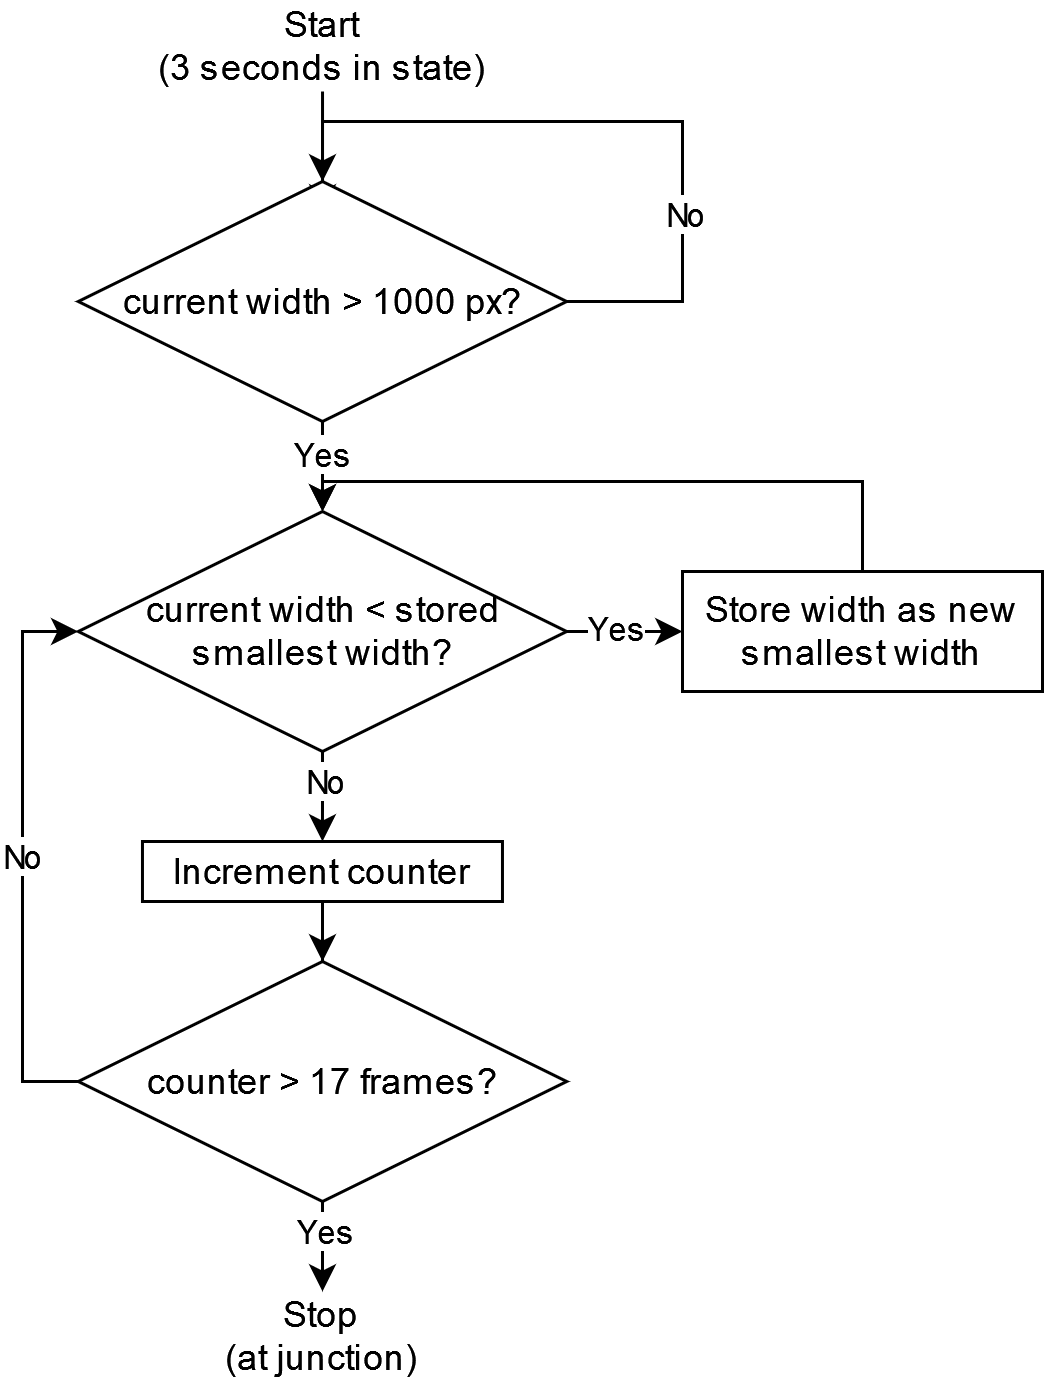
\includegraphics[width=\linewidth]{junctiondiagram.png}
                \caption{Flowchart showing junction detection algorithm based on pavement width.}
                \label{fig:junctionalg}
            \end{figure}

            In the `Junction wait' state, the state machine waits to detect the truck in the appropriate position to safely start the inner loop navigation. Truck detection is based on a very similar methodology as pedestrian pant detection, using HSV colour thresholding followed by erosion, dilation, and contour finding. The state machine will proceed to the next state (moving into the inner loop) once the truck reaches a position in the frame of $x < 400$ pixels and $y<700 $ pixels, a zone that was experimentally determined safe. These values were able be hardcoded becuase the position of the robot when waiting at the junction remained extremely consistant throughout runs. 


            
    \subsection{Navigation Algorithms}
    \subsection{Performance}

\section{License Plate Detection}

\section{Conclusion}

\end{document}